\documentclass[a4paper, 12pt, conference]{IEEEtran}
\usepackage[utf8]{inputenc}
\usepackage[style=ieee]{biblatex}
\usepackage{hyperref}
\usepackage{graphicx}
\usepackage{textcomp}
\usepackage{minted}
\usepackage{tikz}
\usepackage{amsmath}
\usepackage{amssymb}
\usepackage{booktabs}

\title{CS 464 -- Progress Report \\ Breakout Atari\texttrademark{} Game with Reinforcement Learning}
\author{\IEEEauthorblockA{Group 4}\IEEEauthorblockN{Abdullah Arda Aşçı (21702748), Alim Toprak Fırat (21600587), \\ Atahan Yorgancı (21702349), Tuna Alikaşifoğlu (21702125)}}
\date{\today}
\bibliography{bibliography}
\hypersetup{colorlinks=true, allcolors=[rgb]{0.5, 0, 0.5}}

\DeclareMathOperator{\Ex}{\mathbb{E}}

\begin{document}
\maketitle

\section{Introduction}
In our term project we have decided on using reinforcement learning algorithms to learn how to play Atari\texttrademark{} Breakout game.  In Breakout, the player controls a paddle at the bottom of the screen to score by destroying bricks above by hitting a ball in a manner similar to ``pong''. Upon destroying a brick player is awarded a single point of score, and if player misses and the ball goes out bounds the player's life is reduced. From a reinforcement learning perspective classic Atari games like Breakout are suitable RL environments with clearly defined action space, and reward structure for agents.
\begin{figure}[ht]
    \centering{}
    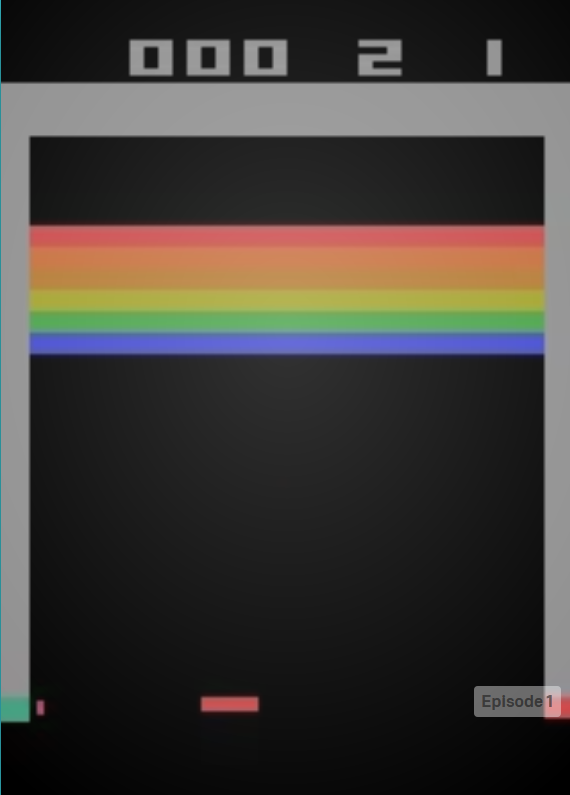
\includegraphics[width=\linewidth, height=0.2\textheight, keepaspectratio]{img/breakout.png}
    \caption{Sample Atari\texttrademark{} Breakout Game with Random Agent~\autocite{breakout}}~\label{fig:breakout}
\end{figure}

More specifically in our project we design and train a deep neural network that can play the nostalgic Atari\texttrademark{} Breakout game. Deep Q-networks (DQN) combine Q-learning with deep neural networks to develop RL agents that can be applied to complex, high dimensional environments, like video games~\autocite{openai}. By receiving rewards and punishments, which are associated with certain in-game actions and outcomes, the agent is expected to develop ``understanding'' of game mechanics such as how to score.

\section{Background Information}
In machine learning, the process of learning is usually separated into 3 categories. Supervised, Unsupervised and Reinforcement learning. In supervised learning, a collection of data instances, and their respective labels are used by the learning algorithm to optimize weight values to be able to create a model which can predict label given features. In unsupervised learning, the unlabeled data is processed in order to perform clustering with respect to certain features, extract underlying patterns, and relations from data. Reinforcement learning doesn't use pre-collected data. Different from other learning methods in reinforcement learning, an agent is placed in an environment which can be interacted with using predefined set of actions, and the agent is trained by receiving rewards or punishments considering the actions of the agent in different states.

In reinforcement learning problems, the agents' past actions influence their current actions by changing the state of the environment. However,agents are not supplied information about which actions to take in a particular situation. The agents learn by maximizing reward (or minimizing punishment) by trying out different combinations from the set of all possible actions after observing the environment.

One of the key concepts in reinforcement learning is the \emph{environment} which maintains the state, and at each time step the learning \emph{agent} observers current state of the environment \(s_t \in S\) where \(S\) is the set of all possible states, and \(s_t\) is the current state in time \(t\). Then, the agent performs an action \(a_t \in A\) depending on the state where \(a_t\) is the current action of the agent, and \(A\) is the possible action space. The environment updates its current state depending on the action of the agent, and outputs the next state \(s_{t+1}\), and \emph{reward} for the state next state \(s_{t+1}\), \(r_{t+1}\). This feedback loop continues until final condition is met, \autoref{fig:rl} demonstrates this interaction between the environment, and the agent.
\begin{figure}
    \centering
    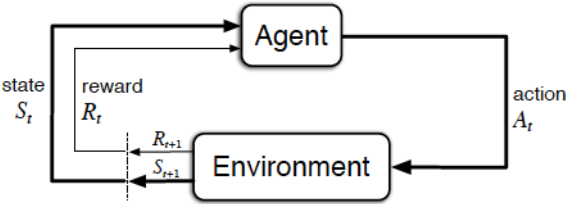
\includegraphics[width=\linewidth]{img/rl.png}
    \caption{RL agent, and environment \cite{sutton2018reinforcement}}
    \label{fig:rl}
\end{figure}

Further, \emph{reward signal}, \(r_a(s,s')\), is the reward for transitioning from state \(s\) to \(s'\) by taking action \(a\). \emph{Value functions}, \(V_{\pi}(s)\), is the total amount of reward is expected from a particular state. While the reward signal is instantaneous, value function calculates the long-term future rewards that can be expected. \emph{Policy}, \(\pi\), is a mapping from the agent's observation of the environment to the set of actions. Informally, the policy of the agent can be considered as the ``strategy'' used by agent to receive more reward. The agent may choose to alter its policy based on how high/low reward it gains from its actions.

RL systems can be broken into two main categories based on whether a \emph{model} of an actual environment is used that are model-based methods, and model-free methods. A \emph{model} of the environment mimics the the behavior of the environment so that the agent can plan what action will result in what kind of outcome. Conversely, in model-free methods, the agent learns by trial-and-error instead of planning out actions \cite{sutton2018reinforcement}.

\subsection{Q-Learning}
Q-learning is a model-free reinforcement learning algorithm. It gives the agents the ability to learn to take optimal actions to move around Markovian state space \cite{watkins1992q}.

Assume there exists an agent and an environment. Let \(\pi: A \times S \to [0,1]\) be the policy map which gives to probability of taking an action in a state. As previously mentioned for time step \(t\) the state of the agent is \(s_t\in S\), and it chooses the action \(a_t\in A\). Define \(\gamma\), where \(0\geq \gamma \geq 1\), to be the \emph{discount factor}. Then, the future discounted return at time $t$ is discounted sum of all future rewards.
\begin{equation}
    R_t=\sum ^T _{t'=t} \gamma^{t'-t}r_{t'}
\end{equation}
where \(T\) is the time step that the game comes to an end. Also define the optimal action-value function as the maximum expected return achievable by taking any action.
\begin{equation}
    Q^*(s,a)=max_{\pi} \Ex [R_t|s_t =s, a_t =a, \pi]
\end{equation}
Since estimating the real value of the action-value function is too costly, a function approximator is used. \(Q(s,a;\theta) \approx Q^*(s,a)\).

Neural networks are an example for a non-linear approximator, with weights \(\theta\). A Q-network is trained to minimize the loss function \(L_i\) which changes at each each epoch.
\begin{equation}
    L_i(\theta_i) = \Ex_{(s,a)}[(y_i-Q(s,a;\theta_i))^2]
\end{equation}
\begin{equation}
    y_i=\Ex_{s'}[r+\gamma max_{a'}Q(s',a';\theta_{i-1})-Q(s,a;\theta_i)|s,a]
\end{equation}
where \(y_i\) is the target which depends on the weights of the neural networks, \(\theta\). Gradient of the loss function with respect to \(\theta\), we get.
\begin{equation}
    \nabla_{\theta_i}L_i(\theta_i)=\Ex_{(s,a),s'}[(r+\gamma max_{a'}Q(s',a';\theta_{i-1})-Q(s,a:\theta_i))\nabla_{\theta_i} Q(s,a;\theta_i)]
\end{equation}
The expected value's calculation can also be too costly, rather than calculating it directly, \emph{stochastic gradient descent} can be used \cite{mnih2013playing}.

\section{Work Done \& Reaming Work}
\subsection{Work Done}
In our proposal, we stated that we would conduct a research on reinforcement learning, deep neural networks and more specific algorithms like Deep Q-networks (DQN) that combines Q-learning with deep neural networks to let reinforcement learning to be  applied to complex, high dimensional environments, like video games~\autocite{openai}. We conducted the promised research to find the optimal approaches to the problem in hand. We informed ourselves on the basics of reinforcement learning and especially on Q-learning with DQN implementations. There are more recent solutions like DeepMind's \textit{Agent57}~\autocite{badia2020agent57} that can outperform DQN based solutions for atari games. However, these type of approaches are necessary for games that have a credit assignment problem, which means that if we choose an action, and we only win or lose hundreds of actions later, leaving us with no idea as to which of our actions led to this win or loss, making it difficult to learn from our actions. The chosen Breakout game is not that complex nor that far-fetched. Thus, our prior research concludes that DQN based solution will be more than sufficient to outperform the atari human benchmark for the Breakout game.

In addition to our background research, we declared that we would obtain a working, playable version of the Breakout game which is suitable for training and testing our artificial agent. In this context, we are utilizing \textit{OpenAI}'s ``Gym'' environments for the implementation of the Breakout atari game. Basically there are two versions of the Breakout game present as a Gym environment. One of the versions provides information of the RAM throughout the game~\autocite{breakout}, and the other provides 3-channel image for each frame throughout the game~\autocite{breakout_image}. Currently both versions of the Breakout game can be initiated from our implementation, and we will decide which one of these versions is the optimum for our case after some experimentation.

At this point of the project, we obtained a playable version of the Breakout game with an human agent, that we call the ``keyboard agent'' by utilizing the example provided in the \textit{GitHub} repo of \texttt{openai/gym}~\autocite{keyboard_agent}. With this aspect of the program, an human agent can play the Breakout atari game by using the keyboard. Version of the game, either RAM based or image based, and the game speed can be adjusted using CLI arguments. In addition to our playable version, we also managed to initialize an artificial agent based version which is suitable for training and testing. Currently, this agent only takes random actions from the action space. However, this environment is crucial for the remaining of the project, and the training and testing will be conducted on this environment, details are provided in the next section.

\subsection{Remaining Work}
At this point we have both RAM and image based Breakout atari game, with an artificial agent and keyboard controlled versions. Currently, artificial agent only takes random actions, but we are planning to thrive on obtaining an artificial agent that outperforms human benchmark. The environments for the reinforcement learning aspect of the project are built, and they are operating successfully. The remaining work is to generate DQN based solution to improve the performance of the artificial agent. In the light of our background research, we believe we can provide an elegant approach. Finally, our research unveils that we should obtain an artificial agent that meets our requirements approximately within 70-96 hours of training.

\section{Work Breakdown Structure}
\begin{table}[h]
    \centering
    \label{tab:task_sharing}
    \caption{Task Sharing}
    \begin{tabular}{rl}\toprule
        \textbf{Worker} & \textbf{Task}\\\midrule
        Abdullah Arda Aşçı & Setting OpenAI, and developing wrappers for \verb+gym+ environment\\
        Atahan Yorgancı & Background research about RL, and DQN\\
        Alim Toprak Fırat & Background research Q-Learning\\
        Tuna Alikaşifoğlu & Developing CLI for running, and training using \verb+gym+ environment\\ \bottomrule
    \end{tabular}
\end{table}

\printbibliography{}

\begin{appendices}
    \onecolumn
    \section{Python Code}
    \inputminted[linenos, fontsize=\scriptsize]{python}{../src/main.py}
\end{appendices}

\end{document}
